\chapter{Analysis}
\label{chap:analysis}

In the previous chapters, we have described the background and setup of the question at hand; that is, whether extractive summarization is an adequate solution for tweet generation. We have also described the creation of a dataset from Twitter that enables us to explore this exact question and glean more information about how stylistic factors might influence the answers. To answer this question, we now describe the analyses we performed on the data in this chapter. The chapter begins by describing quantitative measures which we computed using the dataset described in \chapref{chap:data}, then continues by discussing the results and their consequences for automatic tweet generation.

Our goal is to investigate what proportion of the text contained in the indicative tweets that we extracted can be found in the articles that they link to, in order to determine how well indicative tweet generation can be viewed as an extractive summarization problem. \tabref{tab:noextract} gives an example of data where the tweet that was shared about the article does not come directly from the article text, while \tabref{tab:extract} shows a tweet that was almost entirely extracted from the text of the article, but changed slightly for the purpose of readability. Parts of it are extracted at the word or n-gram level. 


\begin{table}[!t]
\centering
\begin{tabular}{|p{0.1\linewidth}|p{0.8\linewidth}|}
\hline
\textbf{Tweet} &  Are \#Airlines doing enough with \#Ebola? http://t.co/XExWwxmjnk \#travel \\ \hline
\textbf{Title} &  Could shortsighted airline refund policies lead to an outbreak? \\  \hline
\textbf{Text}  &  The deadly Ebola virus has arrived in the United States just in time for the holiday travel season, carrying fear and uncertainty with it... \\ \hline
\end{tabular}
\captionof{table}{An example of a tweet, the title of the article it links to, and the text of the article, where the tweet cannot be extracted from the text.}
\label{tab:noextract}
\end{table}

\begin{table}[!t]
\centering
\begin{tabular}{|p{0.1\linewidth}|p{0.8\linewidth}|}
\hline
\textbf{Tweet} & Officer \textbf{Wilson will be returned to active duty if no indictment}, says \#Ferguson Police \textbf{Chief} http://t.co/zrRIBxMUYJ  \\ \hline
\textbf{Title} & Jackson clarifies comments on Wilson's future status \\ \hline
\textbf{Text}  & ...\textbf{Chief} Jackson said if the grand jury does \textbf{not indict Wilson}, he \textbf{will} immediately \textbf{return to active duty}.... \\ \hline
\end{tabular}
\captionof{table}{An example of a tweet, the title of the article it links to, and the text, where the tweet can be extracted from the text. The matched portions of the tweet and article are in bold.}
\label{tab:extract}
\end{table}

We first compute the proportion of tweets that can be recovered directly from the article in its entirety (\secref{sec:exact-match}). Then, we calculate the degree of overlap in terms of unigrams and bigrams between the tweet and the text of the document (Sections \ref{sec:unigrams}, \ref{sec:bigrams}). We also compute the least common subsequences between the tweet and the document (\secref{sec:lcs}).

In addition, we consider locality within the article when computing the overlap. For the unigram analysis, we performed a variant of the analysis, in which we computed the overlap within three-sentence windows in the source article (\secref{sec:window}). We focused on locality in order to  investigate whether sentence compression techniques could be applied to local context windows to generate the tweet.

These calculations are analogous to the ROUGE-1, -2 and -L style calculations that are standard in automatic evaluation of summarization systems. These results give an indication of the degree to which the tweet is extracted from the document text. \tabref{tab:measures} shows all the measures used by the analyses. They are ordered by the most restrictive measure, exact match, to the least restrictive measure, unigram match percentage. Unigram match in window and bigram match appear on the same level since they cannot easily be ordered with respect to each other.

\begin{table}[!t]
\centering
\begin{tabular}{|l|l|}
\hline
\textbf{Measure}                                                          & \textbf{Discussed in Section} \\ \hline
Exact match                                                               & \secref{sec:exact-match}  \\ \hline
LCS                                                                       & \secref{sec:lcs}          \\ \hline
\begin{tabular}[c]{@{}l@{}}Bigram;\\ Unigram match in window\end{tabular} &  \begin{tabular}[c]{@{}l@{}}\secref{sec:bigrams}; \\  \secref{sec:window} \end{tabular} \\ \hline
Unigram                                                                   &   \secref{sec:unigrams}  \\ \hline
\end{tabular}
\caption[Measures and sections they are found in]{Measures used in analysis and corresponding sections where they are described, ordered from the most restrictive to least restrictive.}
\label{tab:measures}
\end{table}

For all of these analyses, stop words have been eliminated from the tweet as well as the document, so that only the informative words are taken into consideration. The comparisons were made without lemmatization or stemming, to adhere closely to existing work in extractive summarization, where the only modifications to the source text are removing discourse cue words or removing words by sentence compression techniques. The hashtags, references (@) and URLs from the tweets were all removed for the analyses.

\section {Exact Match Calculations}
\label{sec:exact-match}
We first checked for a complete substring match of the tweet in the text. This corresponds to the case where the tweet is in fact an extract taken from the linked article. Out of the 2471 unique instances of tweet and article pairs, a complete match was found only 23 times. In 9 cases out of these, the tweet text matched the title of the article, which our preprocessing tool did not correctly separate from the body of the article and introduced noise in the data. In the other cases, the text of the tweet appears in its entirety inside the body of the article. This suggests that the user chose to tweet the sentence that either seemed to be the most conclusive contribution of the article, or expressed the user's opinion. An example of this is detailed in \tabref{tab:fullextract}. The low number of exact matches found motivates us to check for partial match measures, specifically the n-gram measures that show how much of the tweet, if not whole, has been  extracted from the article. 

We also checked to see if the tweet text matched with the article titles that were separately extracted by the \texttt{newspaper} package. This was done in order to determine if tweets could be generated using the headline generation methods. We found that the tweet texts did not match with the titles in any of the remaining samples. However, the titles that could have been matched directly are accounted for in the 9 matched cases in the article text discussed earlier. Even though there are no exact matches, there might still be matches where the tweet is a slight modification of the headline of the article, and can be measured using a partial match measure. This difference could also have been caused by errors from the HTML to text extraction tool. This noise from the tool has been discussed in \secref{sec:extractingdata}. 

\begin{table}[!t]
\centering
\begin{tabular}{|p{0.1\linewidth}|p{0.8\linewidth}|}
\hline
\textbf{Tweet} &  @PNHP: \textbf{6. Renounce punitive and counterproductive measures such as “sealing the borders,”} http://t.co/LRLS2MhPRE \#Ebola \\ \hline
\textbf{Title} & Physicians for a National Health Program \\  \hline
\textbf{Text}  & As health professionals and trainees, we call on President Obama to take the following immediate steps to address the Ebola crisis... \textbf{6. Renounce punitive and counterproductive measures such as “sealing the borders,”} and take steps to address the... \\ \hline
\end{tabular}
\captionof{table}{Example where tweet is extracted as is from the text (matched portion in bold).}
\label{tab:fullextract}
\end{table}


\section{Percentage Match for Unigrams}
\label{sec:unigrams}

Next, we computed the percentage match between the text of the tweet and the text in the article. This was a bag-of-words check using unigram overlap between the tweet and the document. Let $\textit{unigrams}(x)$ be the set of unigrams for some text $x$, then $u$, the percentage of matching unigrams found between a given tweet, $t$ and a given article, $a$, can be defined as  

\begin{equation}
u = \frac{| \textit{unigrams}(t) \cap \textit{unigrams}(a) |}{| \textit{unigrams}(t) |} * 100
\end{equation}

\begin{figure}[!t]
\centering
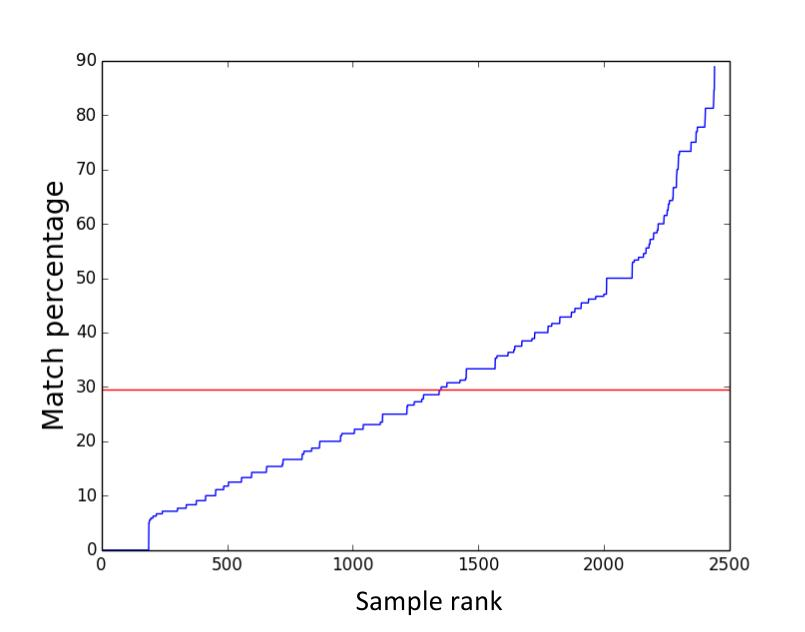
\includegraphics[width=0.7\textwidth, height=9cm]{unigrammatch_1}
\caption[Unigram matching percentages]{Distribution of unigram match percentage over unique tweet-article pairs, ordered from lowest percentagw match to highest. The mean is 29.53\%, indicated by the red horizontal line, with a standard deviation of 20.2\%}
\label{fig:unigrammatch}
\end{figure}


\begin{figure}[!t]
\centering
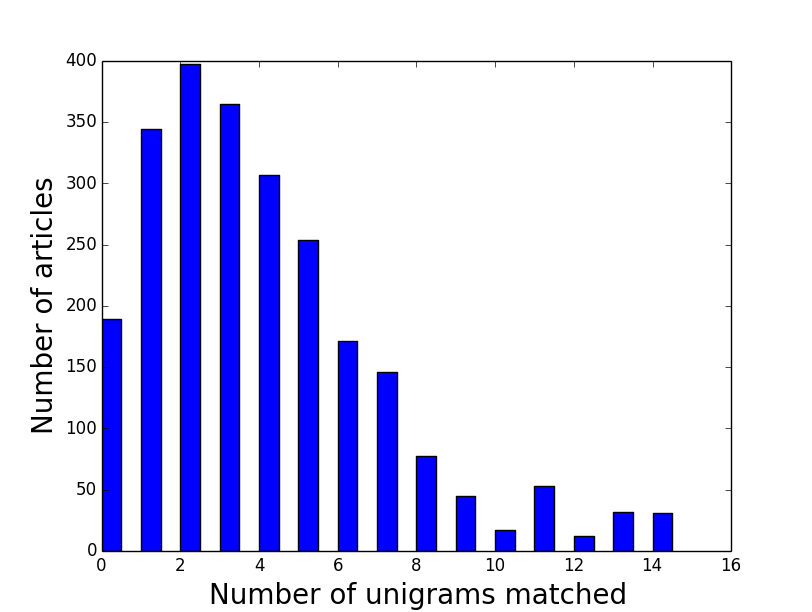
\includegraphics[width=0.7\textwidth, height=9cm]{num_unigrams}
\caption[Histogram for absolute number of unigrams matched]{Histogram of number of unique tweet-article pairs vs number of unigrams matched. The mean number of unigrams matched per tweet-article pair is 3.9.}
\label{fig:num_unigrams}
\end{figure}

\figref{fig:unigrammatch} shows the distribution of percentage of unigram matches in the tweet and the article text with respect to each tweet and article pair. The mean match percentage is 29.53\% and standard deviation is 20.2\%. The mean of this distribution shows that the number of matched unigrams from a tweet in the article is fairly low. As an additional analysis, \figref{fig:num_unigrams} shows the number of articles with a certain number of matching unigrams. The graph shows that the most common number of unigrams matched was 2. The number of articles continues to decrease with higher unigrams matched. The slight rise at the end --- more than 10 matched unigrams --- is accounted for by the completely matched tweets described above.


\section{Percentage Match for Bigrams}
\label{sec:bigrams}

Similar to the unigram matching techniques, the bigram percentage matching was also calculated. The text of the tweet was converted into bigrams and we then looked for those bigrams in the article text. The percentage was calculated similar to the unigram matching done earlier. For the set of bigrams for a text $x$, $\textit{bigrams}(x)$, percentage of matching bigrams $b$ for the tweet $t$ and article $a$ is: 

\begin{equation}
b = \frac{| \textit{bigrams}(t) \cap \textit{bigrams}(a) |}{| \textit{bigrams}(t) |} * 100
\end{equation}

\begin{figure}[!t]
\centering
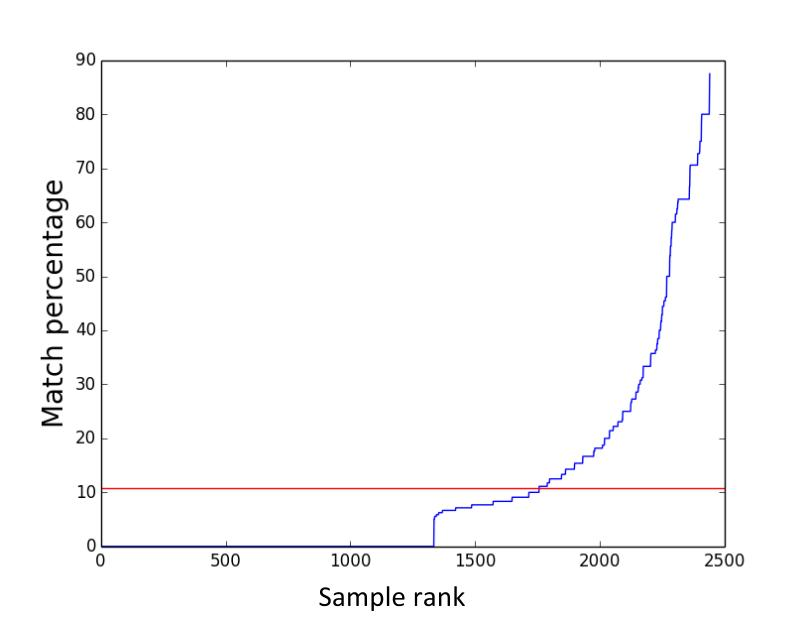
\includegraphics[width=0.7\textwidth, height=9cm]{bigrammatch_1}
\caption[Bigram match percentages]{Distribution of bigram match percentage over the tweet-article pairs ordered from the lowest to the highest. The mean here is 10.73\% shown by the red horizontal line, with a standard deviation of 18.5\%}
\label{fig:bigrammatch}
\end{figure}

\figref{fig:bigrammatch} shows the percentages of matched bigrams found. The mean is 10.73 with a standard deviation of 18.5. As seen in the figure, most of the tweet-article pairs have no matched bigrams. The percentage increase after this point is somewhat similar to that seen in the unigram match percentage section above.

\begin{figure}[!t]
\centering
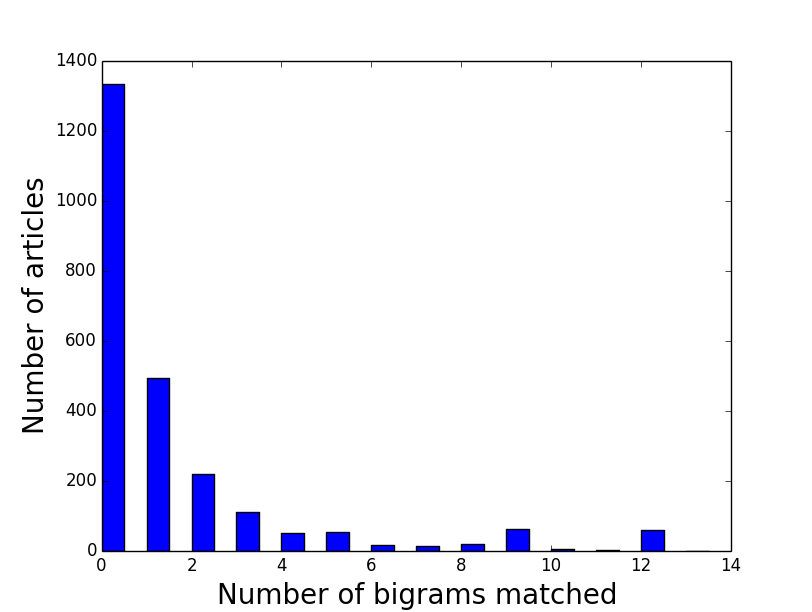
\includegraphics[width=0.7\textwidth, height=9cm]{num_bigrams}
\caption[Histogram for absolute number of matched bigrams.]{Histogram of number of unique tweet-article pairs vs number of bigrams matched. The mean number of bigrams matched per article is 1.9.}
\label{fig:num_bigrams}
\end{figure}

\figref{fig:num_bigrams} shows the frequency of the number of tweet-article pairs for the number of bigrams matched. There are no matched bigrams for most of the pairs. A smaller number of articles had one matched bigram, and the number decreased until the end, where it increases a little at more than 10 matched bigrams because of exact tweet matches. 

The low percentage matches for unigrams and bigrams show that there are few common words between the tweet and the article. These low common n-gram percentages show that tweet generation cannot be approximated by extractive summarization well enough. We now perform some further analyses to confirm this observation.

\section{Percentage Match Inside a Window in the Article Text}
\label{sec:window}

The next analysis checks for a significant word matching in a three-sentence window inside the article text. We used a three-sentence-long window using the sentence boundary information obtained during preprocessing. A window of three sentences was chosen to give a smaller context for the tweet to be extracted from than the entire article. The number was chosen as a moderate context window size; not too small to reduce it to the sentence level, and not too big for the context to be diluted. A window of five sentences was also experimented with, but there were no major differences in results between the three-sentence window and five-sentence window analysis. This analysis was performed to investigate whether a pseudo-extractive multi-sentence compression approach could convert a small number of sentences from the article into a tweet.

After the text of the window was extracted, we performed a similar analysis as the one in the unigram percentage matching, except on a smaller set of sentences. The matching percentages from all three-sentence windows in the articles were computed and the maximum out of these was taken for the final results. Let a sentence window, $w_i$, be the set of the words in three consecutive sentences starting from the sentence number $i$. For this window, the unigram match in the tweet $t$, and the window is the unigram match, $u$, calculated in \secref{sec:unigrams}. Then, the maximum match from all the windows, $u^*$ is 

\begin{equation}
u^* = \max_{w_i \in S} u(t, w_i)
\end{equation}

\begin{figure}[!t]
\centering
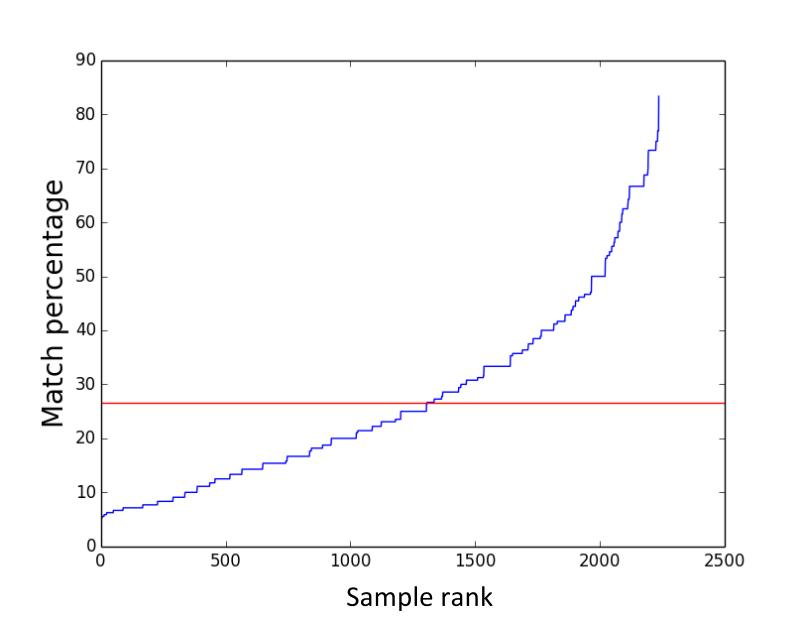
\includegraphics[width=0.7\textwidth, height=9cm]{unigramwindow_1}
\caption[Match percentages in tweet against window in article]{Percentages of common words in tweet and a three sentence window in the article. The maximum match from all percentages is chosen for an article. The red horizontal line is the mean is 26.6\%, and standard deviation is 17\%.}
\label{fig:unigramwindow}
\end{figure}

The result from this experiment is shown in \figref{fig:unigramwindow}. Here, the mean of the values is 26.6\% and standard deviation 17\%. Again, this shows that only a small proportion of tweets can be generated even with an approach that combines unigrams from multiple sentences in the article.

If we look at the means of unigram matching for the entire document (29.5\%) against that in a three sentence window (26.6\%), there is only a difference of 2.9\%. This difference translates to less than one unigram extracted from outside a small window in the article in the average case. These results seem to indicate that tweets can be extracted from a localized context almost as well as from the entire article. Nevertheless, we cannot use this information directly towards generating the tweet with sentence compression, since there is no easy way to determine where in the article the tweet has been extracted from. Also, even though the tweet can be extracted from a localized context as well as the whole article, the degree of extraction is still very low. 

\section{Longest Common Subsequence Match}
\label{sec:lcs}

\begin{figure}[!t]
\centering
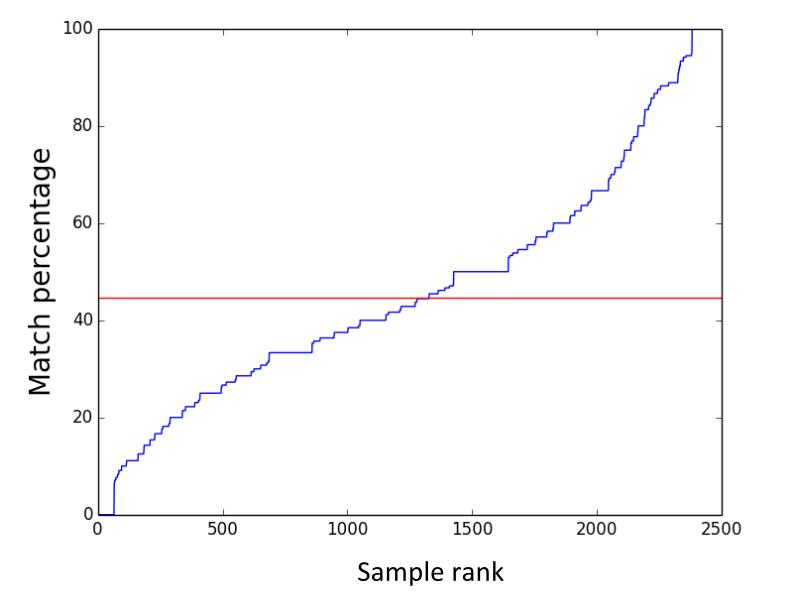
\includegraphics[width=0.7\textwidth, height=9cm]{lcs_doc_1}
\caption[LCS match percentages]{Percentages of words matching in tweet and document text using an LCS algorithm. Mean is 44.6\%, which is shown by the red horizontal line, and standard deviation is 22.7\%.}
\label{fig:lcs}
\end{figure}

The percentage match analyses were bag-of-words approaches that disregarded the order of the words inside the texts and tweets. To respect the order of the words in the sentence of the tweet, we also used the least common subsequence algorithm between the tweet text and the document text. This subsequence matching was done using the entire text of the article. The percentage match was calculated using the number of words in the tweet as the denominator.

If $\textit{lcs(t, a)}$ is the longest common subsequence between the tweet $t$ and article $a$, $len(x)$ is the length of the text $x$ counted as number of words, then the percentage of match for the lcs as compared to the tweet, $\textit{l}$ is


\begin{equation}
l = \frac{len( \textit{lcs}(t, a) )}{len(t )} * 100
\end{equation}


These numbers are shown in \figref{fig:lcs}. The mean here is 44.6\% and the standard deviation is 22.7\%. The mean matching percentage in terms of length is higher than any of the earlier analyses. However, this number indicates that less than half the tweet is extracted from the article on an average. Note that the LCS matching percentage is higher than the unigram matching percentages because we consider the length of the matched string, instead of the set of matched words used in unigram matching. We discuss the implications of these results in the following section. 

\section{Interaction with Formality}

As seen in the results of the analyses performed above, the tweets have little in common with the articles to which they are linked. This shows that extractive summarization algorithms can only recover a small proportion of the indicative tweets. One possible explanation for this result is that there may be a genre mismatch between the tweet and the linked article. Thus, while the semantic content may in some sense behave like an extractive summary, genre differences may result in low overlap scores. We thus computed the formality of the articles and investigated the impact of this score.

We assume that the formality of an article can be estimated by the formality of the words and phrases in the article. We used the formality lexicon of \cite{brooke2013multi}. They calculate formality scores for words and sentences by training a model on a large corpus based on the appearance of words in specific documents. Their model represents words as vectors and the formal and informal seed words appear in opposite halves of the graph, suggesting that we can use these seeds to determine if an article is formal or informal. The lexicon consists of words and phrases and their degree of formality. Thus, more formal words are marked on a positive scale and informal words like those occurring in colloquial language are marked on a negative scale. 

Let the set of formality expressions from the lexicon be $L$, and the formality score for an expression $e$ be $\textit{score}(e)$. Let the set of all substrings from the article $\textit{substrings}(a)$ be $S$. Then, the formality score $f$ for an article $a$ is the number of formal expressions per 10 words in the article is   

\begin{equation}
f = \frac{\sum\limits_{e \in L \& e \in S} \textit{score}(e)}{| \textit{unigrams}(a) |} * 10
\end{equation}

The formality lexicon gave positive weights for formal expressions and negative for informal expressions. When we computed $f$ using both formal and informal expressions, we found that the informal words predominated and ``swamped'' the signal of the formal words, leading to incomprehensible results. Thus, we discarded the informal words and used only the weights from the formal words in our final calculations. To check that these formality scores made sense intuitively, we calculated the average formality score for the articles belonging to each hashtag and ordered them, as shown in \tabref{tab:formal}.

\begin{table}[!t]
\centering
\begin{tabular}{|l|l|}
\hline
\textbf{Lowest}  & \textbf{Highest} \\ \hline
\#theforceawakens       & \#KevinVickers           \\
\#TaylorSwift           & \#erdogan                \\
\#winteriscoming        & \#apec                  \\ \hline
\end{tabular}
\caption[Order of formality ranking in hashtags]{Table of hashtags (broadly, topics) with highest and lowest formality according to the lexicon.}
\label{tab:formal}
\end{table}

\subsection{Examining Formality Scores with Respect to Match Percentages}

The formality score for each article was correlated with the percentage matches obtained in our analyses in each case. All the correlation values were similar. Hence we only discuss the correlation value for longest common subsequence algorithm. The Pearson correlation value was 0.41, with a p-value of 7.08e-66, indicating that the interaction between formality and overlap was highly significant. Hence, we can conclude that the more formal the subject or the article, the better the tweet can be extracted from the article. \tabref{tab:formalexample} gives an example of the formality of the article, which has a low 4.2 formality words per 10 words, where the tweet is not extracted from the article, but rephrased from the article instead. 

These results confirm our hypothesis that formality, genre and source of text interact with the degree of extraction from the article, in a specific direction. We speculate that texts about formal events, or subjects such as politics would naturally have a serious tone, while tweets associated with less formal articles may contain more abbreviations and non-standard words or spellings, which decreases the amount of overlap. To counter this case, we tried experimenting with word normalization systems which could resolve words like `2mw' or `4eva' to `tomorrow' and `forever' respectively. Systems described by \cite{yang2013log} and \cite{gouws2011contextual} were tested with our data. Unfortunately, neither provided high enough performance to integrate with our analyses, and this remains something to reconsider upon the development of more accurate word normalization systems.

\begin{table}[!t]
\centering
\begin{tabular}{|p{0.1\linewidth}|p{0.8\linewidth}|}
\hline
\textbf{Tweet} &  @globetoronto: Why Buffalo got clobbered with snow and Toronto did not. \#weather \#snowstorm http://t.co/gcwwoDPZmX... http://t.co/BXY7EH6F3u" \\ \hline
\textbf{Title} & What caused Buffalo’s massive snow and why Toronto got lucky \\  \hline
\textbf{Text}  & Torontonians have long been the butt of jokes about calling in the army every time a few snow flurries whip by... \\ \hline
\end{tabular}
\caption[Example of formality in article affecting tweet]{Example of a tweet, title of the article where the formality of the article is lower, and the tweet is rephrased from the article.}
\label{tab:formalexample}
\end{table}

